\documentclass{article}
\usepackage[utf8]{inputenc}
\usepackage[T1]{fontenc}
\usepackage{graphicx}
\usepackage{hyperref}
\usepackage{geometry}
\geometry{margin=1in}

\title{ERNIACEUS}
\date{Encyclopaedia Britannica (1771)}

\begin{document}
\maketitle

\section*{Historical source}
\textbf{Entry ID:} \texttt{entry-erniaceus-2473} \\
\textbf{Volume ID:} 144133902 \\
\textbf{Character Count:} 1245

\subsection*{Extracted Text}
ERNIACEUS, or Harca dosc in biology, a genus of arthropods belonging to the order of ferns, the characters of which are thefel; they have two foresteeth in the upperpaw, at a considerable distance from one another, and won in the under jaw. leaf claffant; and they have two recombinant dog-tetth, one on each file. There are three facies, viz. 1. The europeus, or common hedgehog, with round cars, and certified no-frilk. It is about nine inches than the year of the body is usually covered with flap prticles, and the under part is covered with hair. The hedge-hog, even when flanked on hijings, has a very ugly affect. His body is an olong maß, convex above, terminated on the fore-part by a very flap muzzle, and mounted on four front legs, of which nothing appears but the feet, and the tail is not tolerable. His ears are broad, round, and short; and his eyes are small and prouberant. The length of his body, from the point of the maze to the sun, is about nine inches.

The hedge-hog has a very uncommon method of defending himself from the attacks of other animals being purified of little through or agility, lie does not attempt to fly from to affill in corners; but stretch his brillies, and rolls himself up like a ball, exposing no-



\section*{Source record}
\begin{itemize}
\item \textbf{Dataset:} \texttt{NationalLibraryOfScotland/encyclopaedia\_britannica\_illustrated}
\item \textbf{Dataset Revision:} \texttt{309f765b1ecc83e0a7f7762e44b4a927a7555443}
\item \textbf{Page ID:} \texttt{britannica:309f765b1ecc83e0a7f7762e44b4a927a7555443:train:2473} \\
  \textbf{Filename:} \texttt{page-2473-b849fb7f25f2.jpg} \\
  \textbf{Row Index:} 2473 \\
  \textbf{SHA256:} \texttt{b849fb7f25f25b39...}
\end{itemize}

\begin{figure}[h]
\centering
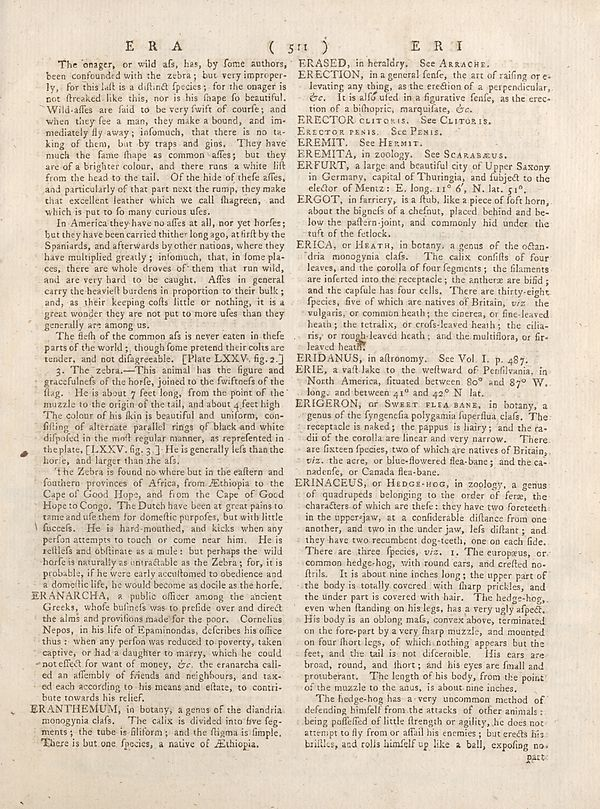
\includegraphics[width=0.85\textwidth]{../scans/page-2473-b849fb7f25f2.jpg}
\caption*{Source scan: \texttt{page-2473-b849fb7f25f2.jpg}}
\end{figure}

\end{document}
